% Template for Cogsci submission with R Markdown

% Stuff changed from original Markdown PLOS Template
\documentclass[10pt, letterpaper]{article}

\usepackage{cogsci}
\usepackage{pslatex}
\usepackage{float}
\usepackage{caption}

% amsmath package, useful for mathematical formulas
\usepackage{amsmath}

% amssymb package, useful for mathematical symbols
\usepackage{amssymb}

% hyperref package, useful for hyperlinks
\usepackage{hyperref}

% graphicx package, useful for including eps and pdf graphics
% include graphics with the command \includegraphics
\usepackage{graphicx}

% Sweave(-like)
\usepackage{fancyvrb}
\DefineVerbatimEnvironment{Sinput}{Verbatim}{fontshape=sl}
\DefineVerbatimEnvironment{Soutput}{Verbatim}{}
\DefineVerbatimEnvironment{Scode}{Verbatim}{fontshape=sl}
\newenvironment{Schunk}{}{}
\DefineVerbatimEnvironment{Code}{Verbatim}{}
\DefineVerbatimEnvironment{CodeInput}{Verbatim}{fontshape=sl}
\DefineVerbatimEnvironment{CodeOutput}{Verbatim}{}
\newenvironment{CodeChunk}{}{}

% cite package, to clean up citations in the main text. Do not remove.
\usepackage{apacite}

% KM added 1/4/18 to allow control of blind submission
\cogscifinalcopy

\usepackage{color}

% Use doublespacing - comment out for single spacing
%\usepackage{setspace}
%\doublespacing


% % Text layout
% \topmargin 0.0cm
% \oddsidemargin 0.5cm
% \evensidemargin 0.5cm
% \textwidth 16cm
% \textheight 21cm

\title{The latent factor structure of child development}

\usepackage{bm}
\usepackage{booktabs}
\usepackage{longtable}
\usepackage{array}
\usepackage{multirow}
\usepackage{wrapfig}
\usepackage{float}
\usepackage{colortbl}
\usepackage{pdflscape}
\usepackage{tabu}
\usepackage{threeparttable}
\usepackage{threeparttablex}
\usepackage[normalem]{ulem}
\usepackage{makecell}
\usepackage{xcolor}

\author{Anonymous Cogsci Submission}

\begin{document}

\maketitle

\begin{abstract}
Hello

\textbf{Keywords:}
one; two;
\end{abstract}

\hypertarget{introduction}{%
\section{Introduction}\label{introduction}}

TO DO

\hypertarget{data}{%
\section{Data}\label{data}}

A child's development can be thought of as the set of developmental
milestones that they have reached at a particular point in time. This
conceptualization results in data with the same structure as the item
response data common to educational measurement. In education, item
response data is most typically students responding to test items (i.e.,
questions) and, in the dichotomous case, getting each question either
correct or incorrect. In the context of child development, the child is
the ``student,'' and each developmental milestone is the ``item.''

We use Kinedu, a Mexico-based child development app, as a source for
this type of data. When parents first start using the Kinedu app, they
are asked a series of questions about which developmental milestones
their child has reached. We consider the 1946 children between 2 and 55
months of age whose parents responded to all 414 of the developmental
milestones. Each developmental miletone on Kinedu is mapped to a
milestone group: physical, cognitive, linguistic, or social \&
emotional. Table \ref{tab:examples} shows the number of developmental
milestones in each group along with an example milestone translated to
English.

\begin{CodeChunk}
\begin{table}[!h]

\caption{\label{tab:examples}Developmental milestone groups and examples}
\centering
\fontsize{8}{10}\selectfont
\begin{tabular}[t]{l|r|l}
\hline
Group & Count & Milestone\\
\hline
Physical & 180 & Stands on their toes\\
\hline
Cognitive & 100 & Finds objects on the floor\\
\hline
Linguistic & 75 & Babbles to imitate conversations\\
\hline
Social \& Emotional & 59 & Complains when play is interrupted\\
\hline
\end{tabular}
\end{table}

\end{CodeChunk}

Figure \ref{fig:growth} shows the age (in months) and number of
developmental milestones for each child. At 12 months old, most children
have reached about 200 developmental milestones. At 24 months old, most
children have reached about 300 developmental milestones. Finally, at 48
months old, most children have reached about 375 of the 414
developmental milestones.

\begin{CodeChunk}
\begin{figure}[tb]
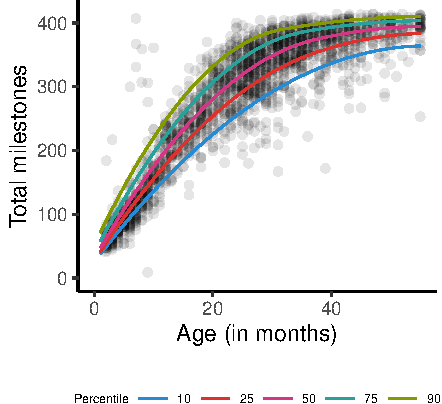
\includegraphics{figs/growth-1} \caption[Number of milestones by age]{Number of milestones by age}\label{fig:growth}
\end{figure}
\end{CodeChunk}

\hypertarget{empirical-assessment-of-the-dimensionality-of-child-development}{%
\section{Empirical assessment of the dimensionality of child
development}\label{empirical-assessment-of-the-dimensionality-of-child-development}}

We frame the assessment of the dimensionality of child development as a
model comparison question.

\hypertarget{models}{%
\subsection{Models}\label{models}}

Item response theory offers a suite of models with which to model item
response data. We adopt the notation used in Chalmers \& others (2012).
Let \(i = 1, \ldots, I\) represent the distinct children and
\(j = 1, \ldots, J\) the developmental milestones. The Kinedu item
response data is stored in a matrix, \(y\), where element \(y_{ij}\)
denotes if the \(i\)th child has or has not achieved the \(j\)th
developmental milestone as reported by their parent/guardian. Each model
represents the \(i\)th child's development using \(m\) latent factors
\(\boldsymbol{\theta}_{i}=(\theta_1, \ldots, \theta_m)\). The \(j\)th
milestone's discriminations (i.e.~slopes)
\(\boldsymbol{a_j}=(a_1, \dots, a_m)\) capture the latent factor
loadings onto that milestone.

We fit four two-parametric logistic (2PL) models where a child's
development is represented by \(m = 1, \ m = 2, \ m = 3,\) and \(m = 4\)
latent factors. According to the 2PL model, the probability of a child
having achieved a developmental milestone is \[
P(y_{ij} = 1 | \boldsymbol{\theta_i}, \boldsymbol{a_j}, b_j) = \sigma(\boldsymbol{a}_{j}^{\top}\boldsymbol{\theta_i} + b_j)
\] where \(b_j\) is the milestone easiness (i.e.~intercept) and
\(\sigma(x) = \frac{e^x}{e^x + 1}\) is the standard logistic function.

The 2PL models learn the latent factor structure entirely from the data,
making them exploratory. The bifactor model offers an alternative
specification where each milestone loads onto a general factor
\(\theta_0\) and a specific factor \(\theta_s\) (Cai, Yang, \& Hansen,
2011). The assignment of each developmental milestone to its specific
factor is an opportunity to specify the latent factor structure, making
the model confirmatory as opposed to exploratory. We map each milestone
to its specific factor according to the four developmental milestone
groups shown in Table X. For the bifactor model, the probability of a
child having achieved a developmental milestone is \[
P(y_{ij} = 1 | \theta_0, \theta_s, a_0, a_s) = \sigma(a_0\theta_0 + a_s\theta_s + b_j).
\]

\hypertarget{model-comparison}{%
\subsection{Model comparison}\label{model-comparison}}

Model comparison in IRT typically uses information criterion such as AIC
and BIC (Maydeu-Olivares, 2013). However, these methods are not
guaranteed to work with modest sample sizes (McDonald \& Mok, 1995).
Instead, we prefer a marginalized version of cross-validation. In
essence, we partition the data into folds based on the children
(i.e.~the rows of the item response matrix). Then for each fold, we
estimate the item parameters using all but that fold, and calculate the
likelihood of that fold by integrating over \(g(\theta)\).

Mathematically and following notation similar to Vehtari, Gelman, \&
Gabry (2017), we partition the data into \(K\) subsets \(y^{(k)}\) for
\(k = 1, \ldots, K\). Each model is fit separately to each training set
\(y^{(-k)}\) yielding item parameter estimates which we compactly denote
\(\Psi_j^{(-k)}\). The predictive (i.e.~out-of-sample) likelihood of
\(y^{(k)}\) is

\[
p(y^{(k)} | y^{(-k)}) = \prod_{i \in i^{(k)}}^{I} \int_\theta \prod_{j=1}^{J} \hat{\text{Pr}}(y_{ij}^{(k)} | \Psi_j^{(-k)}, \theta) g(\theta)d\theta.
\]

The ultimate quantity of interest for each model is the log predictive
likelihood for the entire item response matrix, which is defined as

\[
\text{lpl } y = \sum_{k = 1}^{K} \log p(y^{(k)} | y^{(-k)}).
\]

\hypertarget{results}{%
\subsection{Results}\label{results}}

HELLO

\hypertarget{understanding-the-latent-factor-structure}{%
\subsection{Understanding the latent factor
structure}\label{understanding-the-latent-factor-structure}}

To understand each of the three factors in the best performing model, we
fit the model to the the full dataset. We then estimate the factor
loadings (i.e.~discriminations or slopes) using a varimax rotation. The
varimax rotation results in orthogonal and, therefore, more
interpretable factors (Kaiser, 1959). Figure \ref{fig:factorloadings}
shows the distribution of factor loadings for each group on each of the
three factors. The first factor is mainly cognitive and linguistic. The
second factor is a combination of each of the groups with the strongest
loadings on the physical and social \& emotional milestones. The third
mainly loads positively on linguistic milestones and negatively on
physical milestones.

\textbackslash begin\{CodeChunk\} \textbackslash begin\{CodeOutput\}

Rotation: varimax

Rotated factor loadings:

\begin{verbatim}
               F1       F2        F3     h2
\end{verbatim}

abs\_12 -0.51680 -0.58278 0.044006 0.6087 abs\_148 -0.77483 -0.34897
0.119377 0.7364 abs\_183 -0.60944 -0.57465 0.001097 0.7016 abs\_199
-0.62202 -0.36144 0.086368 0.5250 abs\_203 -0.54057 -0.57353 0.063470
0.6252 abs\_206 -0.56340 -0.50044 -0.046780 0.5700 abs\_317 -0.53209
-0.49228 0.151364 0.5484 abs\_385 -0.79606 -0.26714 0.025069 0.7057
abs\_387 -0.78031 -0.34180 0.085323 0.7330 abs\_69 -0.86880 -0.23527
0.002409 0.8102 attach\_111 -0.23760 -0.35900 -0.059810 0.1889
attach\_122 -0.23534 -0.32500 -0.207071 0.2039 attach\_129 -0.01819
-0.17826 -0.197429 0.0711 attach\_186 -0.19208 -0.18009 0.060800 0.0730
attach\_20 -0.20588 -0.63238 0.100786 0.4524 attach\_252 -0.07626
-0.42677 -0.344363 0.3065 attach\_283 0.15579 -0.19063 -0.208809 0.1042
attach\_308 -0.27002 -0.35564 -0.103310 0.2101 attach\_36 -0.24869
-0.29504 -0.116073 0.1624 attach\_441 -0.76651 -0.35221 -0.003165 0.7116
attach\_97 -0.38659 -0.57228 -0.254446 0.5417 babbling\_126 -0.01834
-0.61770 -0.093935 0.3907 babbling\_143 -0.22360 -0.22116 -0.255054
0.1640 babbling\_196 -0.04657 -0.57924 -0.129663 0.3545 babbling\_197
0.02970 -0.54101 -0.243293 0.3528 babbling\_23 0.19703 -0.54914
-0.210168 0.3846 babbling\_247 0.16482 -0.37034 -0.293189 0.2503
babbling\_301 0.35609 -0.58954 -0.235290 0.5297 babbling\_31 -0.02729
-0.67950 -0.154188 0.4862 babbling\_589 0.12125 -0.62995 -0.090468
0.4197 balance\_635 -0.68247 -0.39343 0.274479 0.6959 balance\_638
-0.73792 -0.24225 0.267574 0.6748 balance\_640 -0.66218 -0.45047
0.277316 0.7183 balance\_641 -0.68935 -0.23409 0.188265 0.5654
balance\_671 -0.63827 -0.26058 0.215091 0.5216 balance\_683 -0.67314
-0.26341 0.163717 0.5493 balance\_708 -0.52089 -0.30648 0.175395 0.3960
balance\_712 -0.57953 -0.29436 0.179695 0.4548 care\_411 -0.71984
-0.33239 0.180054 0.6611 care\_565 -0.76149 -0.44909 0.170122 0.8105
care\_606 -0.64523 -0.36614 0.159087 0.5757 care\_607 -0.59098 -0.25592
0.216885 0.4618 care\_608 -0.75596 -0.27365 0.230677 0.6996 care\_609
-0.64086 -0.30787 0.171594 0.5349 care\_610 -0.79137 -0.18894 0.221224
0.7109 care\_611 -0.72682 -0.19154 0.271319 0.6386 care\_612 -0.78151
-0.17374 0.241659 0.6993 care\_85 -0.74392 -0.29226 0.086208 0.6463
color\_629 -0.63097 -0.25557 0.214753 0.5096 color\_630 -0.84911
-0.22171 0.179524 0.8024 color\_666 -0.84270 -0.14231 0.140191 0.7500
color\_677 -0.84025 -0.15780 0.161535 0.7570 color\_678 -0.79747
-0.16492 0.195257 0.7013 color\_679 -0.82426 -0.15502 0.192348 0.7404
compreh\_109 -0.83074 -0.33811 0.031930 0.8055 compreh\_258 -0.75256
-0.50313 0.034655 0.8207 compreh\_27 -0.79997 -0.29591 -0.054170 0.7304
compreh\_279 -0.85065 -0.35171 0.015058 0.8475 compreh\_307 -0.88603
-0.24551 -0.038121 0.8468 compreh\_32 -0.89737 -0.16569 -0.093742 0.8415
compreh\_360 -0.87122 -0.28877 -0.059089 0.8459 compreh\_366 -0.86884
-0.26314 -0.009213 0.8242 compreh\_368 -0.77041 -0.31750 -0.079296
0.7006 compreh\_505 -0.76775 -0.29606 0.029636 0.6780 compreh\_566
-0.87925 -0.14536 -0.089987 0.8023 compreh\_67 -0.63737 -0.50212
0.063734 0.6624 compreh\_695 -0.72731 -0.11611 0.005496 0.5425
compreh\_700 -0.84840 -0.10520 -0.068342 0.7355 compreh\_703 -0.84802
-0.20975 -0.006219 0.7632 concept\_334 -0.83403 -0.25130 0.055468 0.7618
concept\_386 -0.79878 -0.26368 0.074529 0.7131 concept\_523 -0.87384
-0.24607 0.079225 0.8304 concept\_568 -0.81192 -0.19310 0.086102 0.7039
concept\_569 -0.81951 -0.23228 0.024558 0.7262 concept\_574 -0.75898
-0.24445 0.033444 0.6369 concept\_578 -0.73690 -0.20740 0.117584 0.5999
concept\_579 -0.86886 -0.13312 0.072253 0.7779 concept\_615 -0.78795
-0.29902 0.084420 0.7174 concept\_628 -0.87217 -0.20011 0.047399 0.8030
concept\_659 -0.86026 -0.10987 0.042040 0.7539 concept\_661 -0.86629
-0.17226 0.049797 0.7826 concept\_663 -0.66609 -0.13436 0.025780 0.4624
concept\_665 -0.77878 -0.22300 0.088105 0.6640 concept\_705 -0.87799
-0.21415 0.119316 0.8310 concept\_728 -0.82946 -0.25512 0.066116 0.7575
conver\_617 -0.93844 -0.04204 -0.090258 0.8906 conver\_622 -0.78108
0.00350 -0.090652 0.6183 conver\_623 -0.91920 0.02181 -0.100490 0.8555
conver\_656 -0.93699 -0.01608 -0.115908 0.8916 conver\_657 -0.93419
-0.08356 -0.072035 0.8849 conver\_698 -0.92130 -0.08113 -0.079922 0.8618
conver\_699 -0.93557 -0.05812 -0.051953 0.8814 conver\_704 -0.92432
-0.08615 -0.032960 0.8629 crawl\_116 -0.11104 -0.76023 -0.104203 0.6011
crawl\_158 -0.07378 -0.73756 -0.254467 0.6142 crawl\_164 -0.35155
-0.83977 0.036515 0.8301 crawl\_17 -0.26237 -0.80871 -0.010005 0.7230
crawl\_173 -0.26369 -0.80466 -0.054259 0.7200 crawl\_230 -0.34160
-0.83880 0.015824 0.8205 crawl\_239 -0.09545 -0.66213 -0.245682 0.5079
crawl\_262 -0.25018 -0.77921 -0.083573 0.6767 crawl\_267 -0.10802
-0.74516 -0.180882 0.5996 crawl\_269 -0.17238 -0.80994 -0.186885 0.7206
crawl\_39 -0.35368 -0.80366 0.111123 0.7833 crawl\_413 -0.38707 -0.67677
0.100527 0.6179 crawl\_64 -0.24909 -0.59976 -0.040568 0.4234 crawl\_72
-0.37590 -0.77106 0.049889 0.7383 crawl\_9 -0.10705 -0.67512 -0.199191
0.5069 dfinger\_152 -0.30947 -0.52027 -0.038018 0.3679 dfinger\_172
-0.64064 -0.59371 0.180604 0.7955 dfinger\_235 -0.51083 -0.69929
0.091238 0.7583 dfinger\_251 -0.28863 -0.35764 0.010736 0.2113
dfinger\_295 -0.53841 -0.57700 0.127806 0.6391 dfinger\_296 -0.47415
-0.52538 -0.003304 0.5008 dfinger\_34 -0.71377 -0.43700 0.228969 0.7529
dfinger\_357 -0.64480 -0.53390 0.143884 0.7215 dfinger\_378 -0.53991
-0.56246 0.224670 0.6583 dfinger\_71 -0.63116 -0.47826 0.088819 0.6350
dhand\_135 -0.31368 -0.58140 0.044460 0.4384 dhand\_139 -0.66094
-0.49035 0.259622 0.7447 dhand\_14 -0.58612 -0.37896 0.112273 0.4998
dhand\_140 -0.59072 -0.46000 0.141237 0.5805 dhand\_179 -0.74838
-0.36958 0.188221 0.7321 dhand\_223 -0.51024 -0.51814 0.112738 0.5415
dhand\_298 -0.60587 -0.47915 0.089162 0.6046 dhand\_310 -0.68774
-0.53841 0.188219 0.7983 dhand\_312 -0.69614 -0.27123 0.144895 0.5792
dhand\_314 -0.76173 -0.30605 0.197863 0.7130 dhand\_362 -0.45144
-0.45741 0.083549 0.4200 dhand\_408 -0.57304 -0.51176 0.190849 0.6267
dhand\_467 -0.46787 -0.48098 0.197570 0.4893 dhand\_47 -0.65469 -0.37756
0.267154 0.6425 dhand\_484 -0.42056 -0.35606 0.137612 0.3226 dhand\_57
-0.61070 -0.50855 0.184192 0.6655 dhand\_633 -0.65983 -0.38749 0.270325
0.6586 dindep\_103 -0.71788 -0.40334 0.152031 0.7011 dindep\_241
-0.65652 -0.34404 0.144553 0.5703 dindep\_306 -0.78886 -0.30609 0.176420
0.7471 dindep\_349 -0.40415 -0.46635 0.125270 0.3965 dindep\_461
-0.54799 -0.51333 0.143063 0.5843 dindep\_476 -0.60875 -0.46074 0.160309
0.6086 dindep\_78 -0.44980 -0.29193 0.048769 0.2899 dmemory\_157
-0.65076 -0.35416 -0.082454 0.5557 dmemory\_188 -0.28092 -0.32251
-0.332224 0.2933 dmemory\_28 -0.30324 -0.34468 -0.291086 0.2955
dmemory\_333 -0.13509 -0.13765 -0.298486 0.1263 dmemory\_63 -0.41916
-0.31032 -0.220259 0.3205 dmemory\_89 -0.31540 -0.20928 -0.198568 0.1827
dmemory\_90 -0.31190 -0.14689 -0.298980 0.2082 dmusic\_255 -0.59879
-0.46856 0.009027 0.5782 dmusic\_315 -0.74231 -0.14782 -0.068505 0.5776
dmusic\_338 -0.57017 -0.44865 0.077765 0.5324 dmusic\_417 -0.61885
-0.43087 0.068651 0.5733 dself\_110 -0.42114 -0.58374 -0.065270 0.5224
dself\_120 -0.63540 -0.30396 0.021495 0.4966 dself\_509 -0.81266
-0.18405 -0.010769 0.6944 dself\_95 -0.21487 -0.60574 -0.009816 0.4132
emotion\_451 -0.84304 -0.23617 0.066571 0.7709 emotion\_600 -0.59557
-0.34787 0.020183 0.4761 emotion\_601 -0.57383 -0.28608 0.105462 0.4222
emotion\_602 -0.64693 -0.26997 0.000624 0.4914 emotion\_605 -0.12971
-0.06221 -0.064261 0.0248 emotion\_650 -0.63081 -0.30234 0.098845 0.4991
explore\_102 -0.30849 -0.70286 -0.283390 0.6695 explore\_117 -0.23590
-0.63516 -0.236238 0.5149 explore\_185 -0.40612 -0.66100 0.045118 0.6039
explore\_217 -0.21438 -0.78900 0.081079 0.6751 explore\_281 0.00543
-0.67090 -0.303407 0.5422 explore\_35 -0.20854 -0.75075 -0.004538 0.6071
explore\_37 -0.20681 -0.70676 -0.043110 0.5441 explore\_40 -0.29564
-0.53071 -0.055169 0.3721 explore\_41 0.35021 -0.37610 -0.232980 0.3184
explore\_73 0.21381 -0.48813 -0.106200 0.2953 explore\_81 0.06225
-0.63412 -0.086595 0.4135 explore\_82 -0.02566 -0.44325 -0.194198 0.2348
finger\_463 -0.77837 -0.29464 0.182978 0.7262 finger\_532 -0.78927
-0.22524 0.199986 0.7137 finger\_558 -0.60632 -0.30889 0.179744 0.4953
finger\_631 -0.59887 -0.34157 0.203091 0.5166 finger\_667 -0.80707
-0.18634 0.250304 0.7487 gesture\_22 -0.73264 -0.51714 0.036109 0.8055
gesture\_278 -0.64871 -0.51010 -0.015126 0.6813 gesture\_3 -0.02288
-0.55872 -0.065067 0.3169 gesture\_79 -0.35682 -0.48725 -0.163202 0.3914
gesture\_88 -0.22661 -0.58288 0.047070 0.3933 grammar\_620 -0.89267
-0.03935 -0.121109 0.8131 grammar\_621 -0.88411 -0.14089 -0.031871
0.8025 grammar\_696 -0.90211 -0.06166 -0.112287 0.8302 grammar\_701
-0.67117 -0.21282 -0.012812 0.4959 hand\_414 -0.75635 -0.27660 0.233789
0.7032 hand\_536 -0.81517 -0.25327 0.202245 0.7695 hand\_632 -0.79149
-0.25365 0.247266 0.7519 hand\_634 -0.65068 -0.34322 0.257529 0.6075
hand\_687 -0.77778 -0.24716 0.255843 0.7315 head\_115 -0.25256 -0.51704
-0.137176 0.3499 head\_132 0.02690 -0.25727 -0.179416 0.0991 head\_216
-0.13401 -0.32277 -0.094141 0.1310 head\_30 -0.28549 -0.68385 -0.025746
0.5498 head\_75 -0.07376 -0.49446 -0.110335 0.2621 head\_91 -0.20753
-0.45785 -0.080097 0.2591 Imagine\_329 -0.79649 -0.28882 0.031915 0.7188
Imagine\_475 -0.82278 -0.19867 0.087363 0.7241 Imagine\_625 -0.79422
-0.22474 0.049463 0.6837 Imagine\_645 -0.85186 -0.20665 0.078881 0.7746
Imagine\_646 -0.84643 -0.22799 0.123401 0.7836 Imagine\_647 -0.79822
-0.21957 0.025834 0.6860 Imagine\_651 -0.85414 -0.18135 0.023716 0.7630
Imagine\_707 -0.77938 -0.18431 0.074941 0.6470 imitate\_189 -0.73941
-0.50362 0.051685 0.8030 imitate\_218 -0.55255 -0.27203 -0.159719 0.4048
imitate\_335 -0.79963 -0.28674 -0.057348 0.7249 imitate\_363 -0.73018
-0.31586 -0.013449 0.6331 imitate\_406 -0.69348 -0.47571 0.065450 0.7115
imitate\_443 -0.70540 -0.29966 0.027896 0.5882 imitate\_452 -0.76633
-0.32464 -0.035992 0.6939 imitate\_464 -0.55845 -0.35877 0.003928 0.4406
imitate\_5 -0.61899 -0.47289 0.063172 0.6108 imitate\_53 -0.72577
-0.46658 0.046311 0.7466 imitate\_551 -0.74807 -0.42811 -0.009559 0.7430
imitate\_588 -0.58955 -0.52259 -0.151885 0.6437 indep\_673 -0.61521
-0.23003 0.195635 0.4697 indep\_674 -0.70351 -0.23957 0.238034 0.6090
indep\_675 -0.73792 -0.34410 0.203769 0.7044 indep\_686 -0.65962
-0.23892 0.279137 0.5701 inter\_108 -0.51115 -0.37263 -0.146760 0.4217
inter\_112 -0.24434 -0.54797 0.008303 0.3600 inter\_240 -0.03676
-0.22117 -0.317619 0.1512 inter\_26 0.04140 -0.22981 -0.299402 0.1442
inter\_340 -0.71125 -0.51549 0.048034 0.7739 inter\_354 -0.22722
-0.50497 -0.159145 0.3319 inter\_454 -0.43288 -0.48418 0.024642 0.4224
inter\_51 -0.33070 -0.36975 -0.288733 0.3294 jump\_670 -0.74580 -0.29754
0.286775 0.7270 jump\_680 -0.82880 -0.18018 0.277116 0.7962 jump\_681
-0.77504 -0.12656 0.227203 0.6683 jump\_682 -0.75346 -0.27676 0.260403
0.7121 jump\_706 -0.79468 -0.20487 0.289809 0.7575 jump\_713 -0.74917
-0.29081 0.314067 0.7445 jump\_715 -0.80917 -0.27147 0.277880 0.8057
kick\_168 -0.58525 -0.47296 0.192321 0.6032 kick\_528 -0.74386 -0.37167
0.256035 0.7570 kick\_642 -0.64909 -0.33087 0.253715 0.5952 kick\_643
-0.73177 -0.38029 0.264351 0.7500 kick\_714 -0.61106 -0.34817 0.265703
0.5652 memory\_19 -0.80137 -0.38548 0.069265 0.7956 memory\_421 -0.82079
-0.35578 0.030471 0.8012 memory\_435 -0.82658 -0.17295 -0.083011 0.7200
memory\_436 -0.51936 -0.23053 -0.054047 0.3258 memory\_472 -0.76943
-0.31820 0.014306 0.6935 memory\_478 -0.84481 -0.17671 -0.034799 0.7461
memory\_524 -0.85426 -0.16151 -0.048335 0.7582 memory\_613 -0.78525
-0.33762 0.102208 0.7410 memory\_627 -0.81539 -0.23578 -0.004477 0.7205
memory\_664 -0.83838 -0.20419 0.013822 0.7448 move\_1 -0.25649 -0.77474
-0.010334 0.6661 move\_114 -0.10789 -0.71923 -0.003777 0.5289 move\_130
-0.30672 -0.51057 0.085440 0.3621 move\_133 -0.40593 -0.55777 0.006601
0.4759 move\_146 -0.16985 -0.44974 -0.105350 0.2422 move\_149 -0.11143
-0.73172 0.004735 0.5479 move\_153 -0.21642 -0.86206 0.197434 0.8290
move\_159 -0.10137 -0.51849 -0.176788 0.3104 move\_165 -0.34304 -0.77071
0.087298 0.7193 move\_207 -0.04477 -0.40226 -0.024879 0.1644 move\_288
-0.29735 -0.64061 0.018620 0.4991 move\_294 -0.11344 -0.70484 0.037914
0.5111 move\_299 -0.22245 -0.69838 -0.017745 0.5375 move\_86 0.16859
-0.37996 -0.213382 0.2183 music\_352 -0.78063 -0.23336 0.039766 0.6654
music\_468 -0.66147 -0.21850 0.037773 0.4867 music\_537 -0.85428
-0.05421 -0.066689 0.7372 music\_655 -0.86011 -0.01980 -0.054284 0.7431
newborn\_131 0.15394 -0.23865 -0.261474 0.1490 newborn\_136 0.13158
-0.31932 -0.308159 0.2142 newborn\_150 0.03536 -0.18037 -0.220922 0.0826
newborn\_193 0.08219 -0.25083 -0.201681 0.1103 newborn\_201 -0.03314
-0.13060 -0.162080 0.0444 newborn\_21 -0.13688 -0.28194 -0.162996 0.1248
newborn\_236 0.09735 -0.17050 -0.237761 0.0951 newborn\_285 0.02998
-0.15195 -0.233612 0.0786 newborn\_289 0.08493 -0.22928 -0.300269 0.1499
newborn\_43 0.06656 -0.36740 -0.266369 0.2104 problem\_409 -0.71081
-0.27185 0.160110 0.6048 problem\_624 -0.65174 -0.35570 0.133339 0.5691
problem\_626 -0.77449 -0.25373 0.170742 0.6934 problem\_662 -0.59130
-0.25913 0.054810 0.4198 problem\_669 -0.72710 -0.21314 0.182396 0.6074
prod\_419 -0.91900 -0.03064 -0.143428 0.8661 prod\_465 -0.91184 -0.13097
-0.124980 0.8642 prod\_483 -0.93286 -0.01455 -0.122331 0.8854 prod\_527
-0.90502 -0.11902 -0.041584 0.8350 prod\_540 -0.76236 -0.17400 -0.141680
0.6315 prod\_544 -0.91625 -0.05138 -0.117634 0.8560 prod\_564 -0.91308
-0.11127 -0.083298 0.8530 prod\_572 -0.90990 -0.05347 -0.136354 0.8494
pronoun\_391 -0.82980 -0.11075 -0.203992 0.7424 pronoun\_394 -0.87368
-0.10156 -0.185804 0.8081 pronoun\_490 -0.68382 -0.16827 -0.121986
0.5108 pronoun\_587 -0.86451 -0.01878 -0.191532 0.7844 pronoun\_688
-0.86463 -0.05043 -0.153052 0.7735 pronoun\_689 -0.86222 -0.04727
-0.147430 0.7674 pronoun\_690 -0.79422 -0.04742 -0.092606 0.6416
pronoun\_691 -0.83273 -0.03756 -0.134896 0.7131 pronoun\_692 -0.85976
-0.02751 -0.167505 0.7680 pronoun\_693 -0.84794 -0.05947 -0.138355
0.7417 relation\_619 -0.80794 -0.12863 -0.062645 0.6732 relation\_648
-0.43180 -0.30943 0.049950 0.2847 relation\_649 -0.45181 -0.39761
0.055438 0.3653 relation\_694 -0.60133 -0.34735 0.003749 0.4823
relation\_84 -0.37381 -0.40225 0.087247 0.3091 run\_637 -0.74455
-0.43411 0.281636 0.8221 run\_711 -0.82411 -0.32618 0.328455 0.8934
run\_721 -0.62137 -0.34187 0.228998 0.5554 run\_723 -0.67167 -0.35261
0.243492 0.6348 run\_725 -0.65397 -0.35414 0.291894 0.6383 run\_726
-0.75445 -0.33216 0.345903 0.7992 run\_727 -0.78941 -0.36483 0.267860
0.8280 scrib\_330 -0.50138 -0.46482 0.172502 0.4972 scrib\_377 -0.48003
-0.56073 0.173518 0.5750 scrib\_481 -0.61539 -0.33095 0.208608 0.5317
scrib\_516 -0.70865 -0.34658 0.185030 0.6565 scrib\_518 -0.70703
-0.33653 0.172910 0.6430 scrib\_519 -0.75983 -0.26339 0.212147 0.6917
scrib\_559 -0.68848 -0.36513 0.197957 0.6465 self\_603 -0.73496 -0.28367
0.091723 0.6291 self\_618 -0.91067 -0.04858 -0.050417 0.8342 self\_653
-0.90629 -0.08695 -0.107573 0.8405 self\_658 -0.91740 0.00107 -0.091571
0.8500 senses\_138 -0.53163 -0.25761 -0.371878 0.4873 senses\_144
-0.11080 -0.28714 -0.344842 0.2136 senses\_145 -0.27109 -0.55199
-0.296297 0.4660 senses\_212 -0.38546 -0.32213 -0.133449 0.2702
senses\_214 -0.23047 -0.32015 -0.183881 0.1894 senses\_243 -0.48732
-0.24346 -0.115004 0.3100 senses\_303 -0.10882 -0.28717 -0.416676 0.2679
senses\_304 -0.43548 -0.13717 -0.100307 0.2185 senses\_38 0.08274
-0.14217 -0.199517 0.0669 senses\_577 -0.39413 -0.50233 0.039061 0.4092
senses\_6 -0.20941 -0.40904 -0.219205 0.2592 senses\_93 -0.27825
-0.21354 -0.069720 0.1279 shapes\_396 -0.86533 -0.11358 0.073181 0.7671
shapes\_397 -0.87163 -0.12943 0.073097 0.7818 shapes\_398 -0.87673
-0.14244 0.086914 0.7965 shapes\_399 -0.88285 -0.12244 0.088169 0.8022
shapes\_427 -0.88796 -0.03677 0.019242 0.7902 shapes\_429 -0.87530
-0.15893 0.123530 0.8067 shapes\_430 -0.81969 -0.12291 0.092841 0.6956
shapes\_431 -0.82982 -0.14239 0.110102 0.7210 shapes\_502 -0.86349
-0.23439 0.168516 0.8289 shapes\_503 -0.82046 -0.18519 0.146524 0.7289
shapes\_521 -0.88792 -0.17512 0.100310 0.8291 shapes\_660 -0.89847
-0.12306 0.066866 0.8269 sitting\_118 -0.41699 -0.77118 0.108220 0.7803
sitting\_151 -0.35771 -0.65760 0.068490 0.5651 sitting\_160 -0.30939
-0.57811 -0.037519 0.4313 sitting\_162 0.00407 -0.60536 -0.177203 0.3979
sitting\_227 -0.01430 -0.60573 -0.076956 0.3730 sitting\_270 -0.51735
-0.72748 0.188113 0.8323 sitting\_272 -0.19567 -0.57296 -0.072943 0.3719
sitting\_33 -0.01823 -0.46609 -0.150684 0.2403 sitting\_92 -0.43001
-0.64712 0.083659 0.6107 standing\_113 -0.41478 -0.76007 0.169243 0.7784
standing\_208 -0.59154 -0.64677 0.317316 0.8689 standing\_209 -0.54853
-0.64767 0.167364 0.7484 standing\_245 -0.47631 -0.69602 0.206391 0.7539
standing\_271 -0.17725 -0.58876 -0.016846 0.3783 standing\_325 -0.62938
-0.55131 0.297733 0.7887 standing\_350 -0.69098 -0.51985 0.323909 0.8526
standing\_438 -0.65127 -0.54868 0.351565 0.8488 standing\_459 -0.69313
-0.50986 0.329312 0.8488 standing\_470 -0.67139 -0.52038 0.351033 0.8448
steps\_124 -0.33700 -0.68834 0.107535 0.5989 steps\_15 -0.12503 -0.64711
-0.070198 0.4393 steps\_16 -0.66264 -0.61743 0.267613 0.8919 steps\_309
-0.73323 -0.47663 0.332452 0.8753 steps\_355 -0.59069 -0.64577 0.263696
0.8355 steps\_4 -0.63048 -0.54870 0.393996 0.8538 steps\_415 -0.53416
-0.61373 0.206056 0.7044 throw\_456 -0.63879 -0.35951 0.240175 0.5950
throw\_457 -0.71088 -0.48364 0.291987 0.8245 throw\_458 -0.63159
-0.38259 0.222453 0.5948 throw\_529 -0.60432 -0.33654 0.176118 0.5095
throw\_530 -0.50243 -0.32162 0.235224 0.4112 throw\_644 -0.62198
-0.32936 0.214171 0.5412 throw\_672 -0.59106 -0.31941 0.245875 0.5118
throw\_716 -0.58665 -0.33365 0.226027 0.5066 throw\_717 -0.63433
-0.28103 0.251128 0.5444 throw\_718 -0.47945 -0.29647 0.245500 0.3780
walk\_182 -0.67615 -0.46837 0.325353 0.7824 walk\_382 -0.53664 -0.60750
0.276979 0.7338 walk\_471 -0.58521 -0.54243 0.280812 0.7156 walk\_538
-0.72923 -0.45487 0.278307 0.8161 walk\_639 -0.69834 -0.35391 0.290175
0.6971 walk\_676 -0.73628 -0.26597 0.257621 0.6792 walk\_684 -0.63499
-0.44943 0.217972 0.6527 walk\_685 -0.68929 -0.38416 0.226307 0.6739
walk\_709 -0.69429 -0.31448 0.296527 0.6689 walk\_710 -0.72521 -0.27748
0.268015 0.6748 words\_24 -0.79808 -0.23025 -0.150630 0.7126 words\_249
-0.78007 -0.32015 -0.083887 0.7180 words\_353 -0.88525 -0.09676
-0.218593 0.8408 words\_373 -0.89474 -0.06526 -0.164544 0.8319
words\_375 -0.81848 -0.16940 -0.136419 0.7172 words\_437 -0.92674
-0.07124 -0.161292 0.8899 words\_439 -0.85292 -0.15842 -0.108072 0.7643
words\_445 -0.91155 -0.12918 -0.144866 0.8686 words\_469 -0.92259
0.00185 -0.143191 0.8717 words\_534 -0.89222 -0.07983 -0.067816 0.8070
words\_54 -0.75873 -0.19707 -0.211569 0.6593 words\_55 -0.85537 -0.24372
-0.047173 0.7933 words\_573 -0.93519 -0.01089 -0.134006 0.8926
words\_614 -0.91353 -0.09142 -0.193700 0.8804 words\_7 -0.67352 -0.26548
-0.303189 0.6160 words\_702 -0.63849 -0.10040 -0.334253 0.5295

Rotated SS loadings: 168.336 67.452 12.188

Factor correlations:

F1 F2 F3 F1 1 0 0 F2 0 1 0 F3 0 0 1 \textbackslash end\{CodeOutput\}

\begin{figure}[tb]
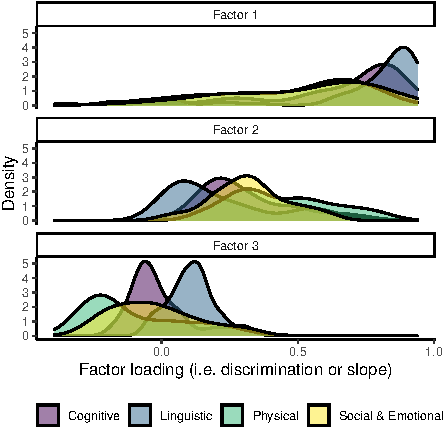
\includegraphics{figs/factorloadings-1} \caption[Factor loadings by group]{Factor loadings by group}\label{fig:factorloadings}
\end{figure}

\textbackslash end\{CodeChunk\}

We also estimate the factor scores for each child using expected a
posteriori (EAP) with a three dimensional standard normal distribution
(Embretson \& Reise, 2013). Figure \ref{fig:factorscores} shows the
relationship between age and factor score for each factor. The first
factor, perhaps unsurprisingly, has a high correlation (r = 0.90) with
age. The second factor has a strong association with age from 2 to 16
months but thereafter is unrelated to age. By and large, the third
factor does not have any association with age.

\begin{CodeChunk}
\begin{figure}[tb]
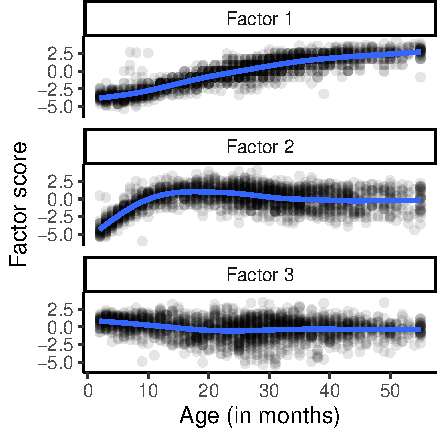
\includegraphics{figs/factorscores-1} \caption[The first factor is highly associated with age]{The first factor is highly associated with age}\label{fig:factorscores}
\end{figure}
\end{CodeChunk}

\hypertarget{acknowledgements}{%
\section{Acknowledgements}\label{acknowledgements}}

We'd like to thank Kinedu for providing the data that made this research
possible.

\hypertarget{references}{%
\section{References}\label{references}}

\setlength{\parindent}{-0.1in} 
\setlength{\leftskip}{0.125in}

\noindent

\hypertarget{refs}{}
\leavevmode\hypertarget{ref-cai2011generalized}{}%
Cai, L., Yang, J. S., \& Hansen, M. (2011). Generalized full-information
item bifactor analysis. \emph{Psychological Methods}, \emph{16}(3), 221.

\leavevmode\hypertarget{ref-chalmers2012mirt}{}%
Chalmers, R. P., \& others. (2012). Mirt: A multidimensional item
response theory package for the r environment. \emph{Journal of
Statistical Software}, \emph{48}(6), 1--29.

\leavevmode\hypertarget{ref-embretson2013item}{}%
Embretson, S. E., \& Reise, S. P. (2013). \emph{Item response theory}.
Psychology Press.

\leavevmode\hypertarget{ref-kaiser1959computer}{}%
Kaiser, H. F. (1959). Computer program for varimax rotation in factor
analysis. \emph{Educational and Psychological Measurement},
\emph{19}(3), 413--420.

\leavevmode\hypertarget{ref-maydeu2013goodness}{}%
Maydeu-Olivares, A. (2013). Goodness-of-fit assessment of item response
theory models. \emph{Measurement: Interdisciplinary Research and
Perspectives}, \emph{11}(3), 71--101.

\leavevmode\hypertarget{ref-mcdonald1995goodness}{}%
McDonald, R. P., \& Mok, M. M.-C. (1995). Goodness of fit in item
response models. \emph{Multivariate Behavioral Research}, \emph{30}(1),
23--40.

\leavevmode\hypertarget{ref-vehtari2017practical}{}%
Vehtari, A., Gelman, A., \& Gabry, J. (2017). Practical bayesian model
evaluation using leave-one-out cross-validation and waic.
\emph{Statistics and Computing}, \emph{27}(5), 1413--1432.

\bibliographystyle{apacite}


\end{document}
